\documentclass[varwidth, border=0pt]{standalone}

\usepackage{times}      % Loads the Times-Roman Fonts
\usepackage{mathptmx}   % Loads the Times-Roman Math Fonts
\usepackage{subcaption}
\usepackage[labelfont={bf,sf},%
labelsep=period,%
justification=centering,
labelformat=parens,labelsep=quad,skip=3pt,font=scriptsize]{caption}
\usepackage{graphicx}

\begin{document}
	
	\begin{figure}
	\centering
\begin{subfigure}{0.5\linewidth}
	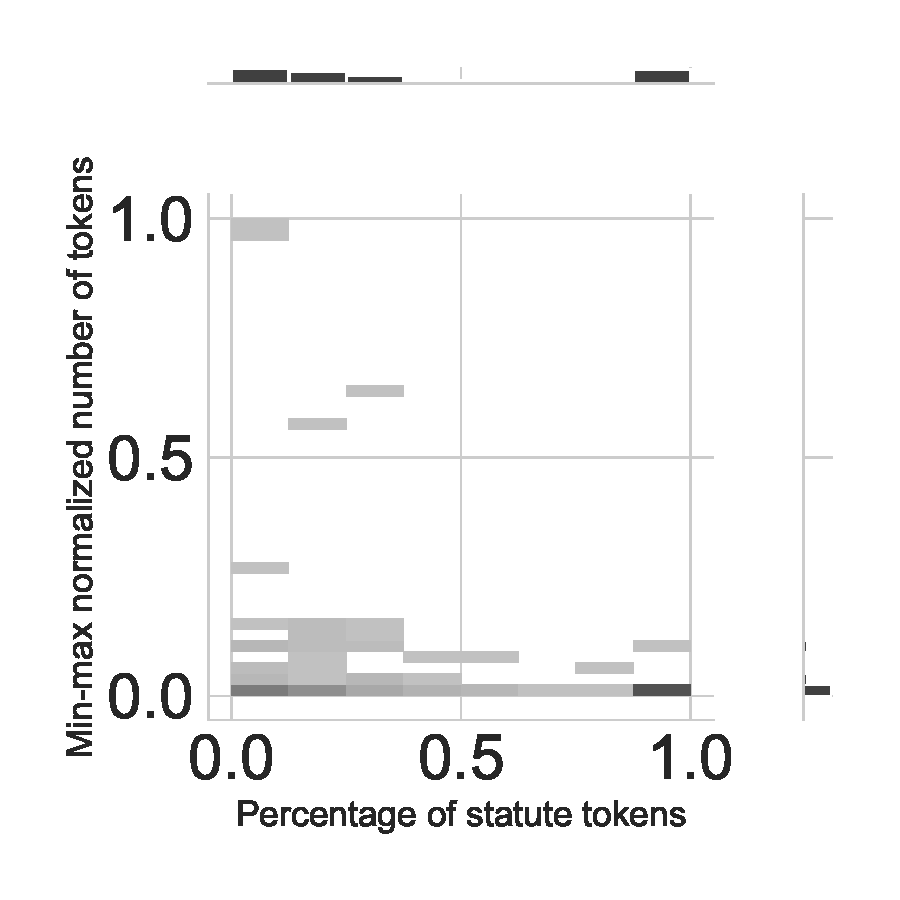
\includegraphics[width=\linewidth]{../../graphics/family-compositions/family-hist2d-us-2019.pdf}~%
	\subcaption{United States}
\end{subfigure}%
~
\begin{subfigure}{0.5\linewidth}
	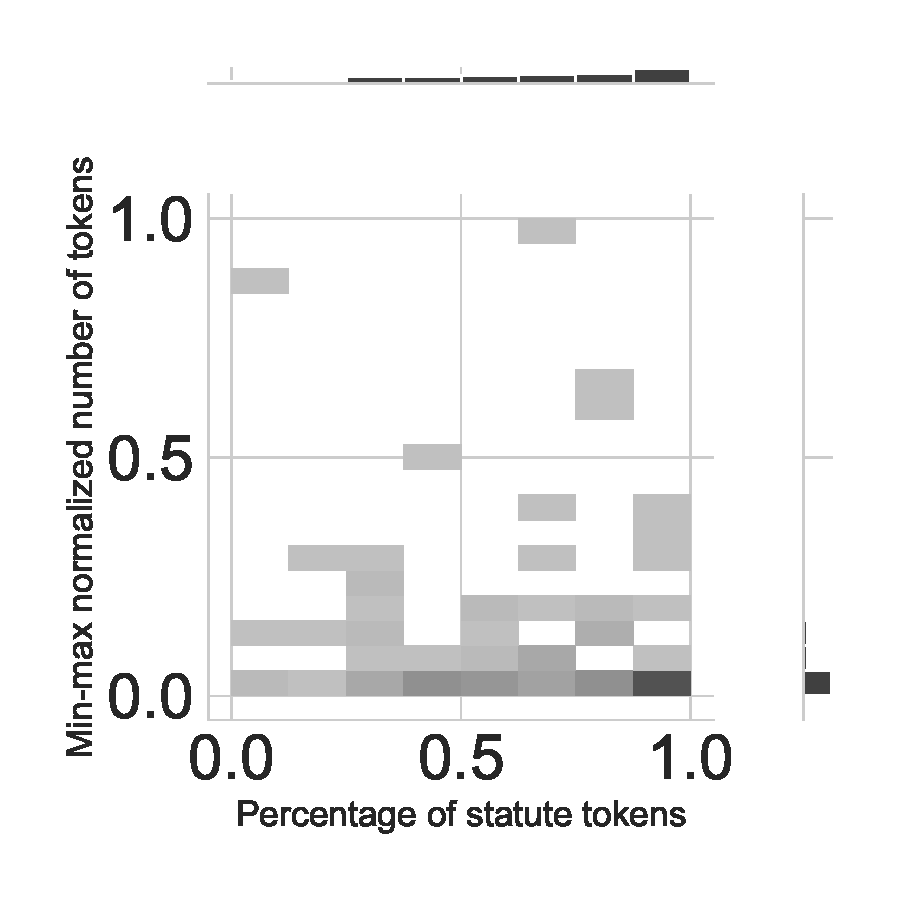
\includegraphics[width=\linewidth]{../../graphics/family-compositions/family-hist2d-de-2019.pdf}~%
	\subcaption{Germany}
\end{subfigure}
	\end{figure}
	
\end{document}